 \subsection{Visualize the list of scheduled runs}
Into the page of \emph{Track4Run} a User can perform a manual search specifying the characteristics (location range and minimum/maximum distance) of the scheduled runs that wants to visualize. Then the System will show the list of scheduled runs that meet the User's specifications. 

\begin{table}[H]
	\centering
    
    \begin{tabular}{|p{3.5cm}|p{10.3cm}|}
    
    \hline
    \textbf{\large{Actors}}  			& \tabitem User 	\\
    				 					
    \hline
    \textbf{\large{Goals}} 				& \ref{goal:run3}\\
    
    \hline
    \textbf{\large{Enter Condition}}	& The \emph{User} is already logged in.		\\
    
    \hline
    \textbf{\large{Events Flow}}		& \begin{enumerate}[leftmargin=0.5cm]
                                          	\item The \emph{User} specifies the characteristics of the run that wants to visualize(if not specified the System will show all the scheduled runs)  
                                          	 \item The System shows the list of scheduled runs that meet the required features
                                          \end{enumerate}
    										\\
    \hline
    \textbf{\large{Exit Conditions}}    & The list of scheduled runs, that correspond to the user's choice, is shown.  \\
    
    \hline
    \textbf{\large{Exceptions}} 		& \\
    
    \hline
    
    
    \end{tabular}
	
\end{table}

\begin{figure}[H]
    \centering
    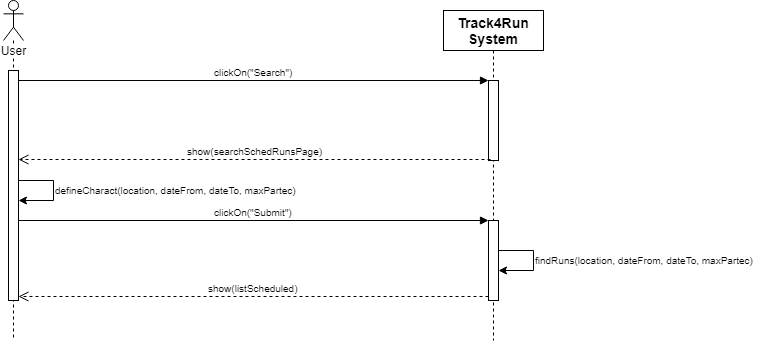
\includegraphics[scale=0.4]{Pictures/visListSchedRunsSeqDiag.png}
    \caption{State chart  \emph{Data4Help} System}
\end{figure}
